% ============================================================
% Minimización sin Restricciones
% Boyd & Vandenberghe — Capítulo 9
% Presentación Beamer introductoria
% Curso: MM-520 Programación Matemática II
% ============================================================
\documentclass[10pt,aspectratio=169]{beamer}

% --- Paquetes ---
\usepackage[utf8]{inputenc}
\usepackage[T1]{fontenc}
\usepackage[spanish]{babel}
\usepackage{amsmath, amssymb, amsthm, mathtools}
\usepackage{tikz}
\usetikzlibrary{calc,arrows.meta,positioning,shapes.geometric,backgrounds,fit}
\usepackage{graphicx}
\usepackage{booktabs}
\usepackage{xcolor}

% --- Tema y colores (mismo estilo que cap4) ---
\usetheme{Madrid}
\usecolortheme{seahorse}
\definecolor{accentblue}{RGB}{31,73,125}
\definecolor{accentgreen}{RGB}{46,125,50}
\definecolor{accentred}{RGB}{198,40,40}
\definecolor{accentorange}{RGB}{230,120,30}
\setbeamercolor{frametitle}{bg=accentblue,fg=white}
\setbeamercolor{title}{fg=accentblue}
\setbeamertemplate{navigation symbols}{}
\setbeamertemplate{footline}[frame number]

% --- Datos del documento ---
\title{Minimización sin Restricciones}
\subtitle{Capítulo 9 --- Boyd \& Vandenberghe}
\author{Optimización Convexa --- MM-520}
\date{\today}

% --- Atajos ---
\newcommand{\R}{\mathbb{R}}
\newcommand{\N}{\mathbb{N}}
\newcommand{\x}{\mathbf{x}}
\newcommand{\g}{\nabla f}
\newcommand{\Hess}{\nabla^{2} f}
\newcommand{\dom}{\operatorname{dom}}
\newcommand{\epi}{\operatorname{epi}}
\newcommand{\aff}{\operatorname{aff}}
\newcommand{\argmin}{\operatorname*{arg\,min}}
\renewcommand{\vec}[1]{\mathbf{#1}}

% ============================================================
\begin{document}

% ============================================================
\begin{frame}
  \titlepage
\end{frame}

% ------------------------------------------------------------
\section{Esquema del capítulo}
% ------------------------------------------------------------
\begin{frame}{Esquema del capítulo}
  \tableofcontents
\end{frame}

% ============================================================
\section{El problema de minimización sin restricciones}
% ============================================================
\begin{frame}{9.1 El problema}
  \begin{block}{Problema}
    \[
      \min_{x \in \R^{n}} f(x)
    \]
    donde $f:\R^{n}\to\R$ es \emph{dos veces continuamente diferenciable}
    ($f \in \mathcal{C}^{2}$), y el dominio $\dom f$ es \textbf{todo} $\R^{n}$
    (o abierto y la función se extiende suavemente).
  \end{block}
  \begin{itemize}
    \item \textbf{Óptimo global:} $x^{\star}$ con $f(x^{\star}) \le f(x)$ para todo $x$.
    \item \textbf{Óptimo local:} $f(x) \ge f(x^{\star})$ para $x$ en un entorno de $x^{\star}$.
    \item \textbf{Condición necesaria} (1\textsuperscript{er} orden): si $x^{\star}$ es local y $f$ diferenciable,
          \[
            \nabla f(x^{\star}) = 0.
          \]
    \item \textbf{Condición suficiente} (2.\textsuperscript{o} orden): si $\nabla f(x^{\star}) = 0$ y
          $\nabla^{2}f(x^{\star}) \succ 0$ (definida positiva), entonces $x^{\star}$ es \emph{estricto} local.
  \end{itemize}
\end{frame}

\begin{frame}{9.1 Ejemplo: cuadrática diagonal}
  \begin{columns}[T]
    \begin{column}{0.55\textwidth}
      \begin{example}
        $f(x) = \tfrac{1}{2}(x_1^2 + \gamma\, x_2^2)$ con $\gamma > 0$.
        \[
          \nabla f(x) = \begin{pmatrix} x_1 \\ \gamma\, x_2 \end{pmatrix},
          \qquad
          \nabla^2 f(x) = \begin{pmatrix} 1 & 0 \\ 0 & \gamma \end{pmatrix}.
        \]
        El único punto crítico es $x^\star = (0,0)$ y la Hessiana es
        definida positiva, así que $x^\star$ es un \textbf{mínimo global estricto}.
      \end{example}
      \begin{itemize}
        \item Si $\gamma \gg 1$: \emph{valle estrecho} (mal condicionado).
        \item Si $\gamma = 1$: contornos circulares (bien condicionado).
      \end{itemize}
    \end{column}
    \begin{column}{0.45\textwidth}
      \begin{center}
        \begin{tikzpicture}[scale=0.55, every node/.style={font=\scriptsize}]
          \draw[->] (-4.2,0)--(4.5,0) node[right]{$x_1$};
          \draw[->] (0,-4.2)--(0,4.5) node[above]{$x_2$};
          % valley along x1 axis (gamma large)
          \foreach \r in {0.6,1.2,1.8,2.4,3.0,3.6} {
            \draw[accentblue!60, thick] ({\r*0.97},0) ellipse ({\r*0.97} and {\r*0.18});
          }
          \draw[accentred,->,thick] (2.6,0) -- (-3.0,0);
          \node[accentblue] at (0,3.6) {contornos $f(x)=c$};
          \node[accentred] at (-2.2,-0.7) {valle};
        \end{tikzpicture}
      \end{center}
    \end{column}
  \end{columns}
\end{frame}

% ============================================================
\section{Algoritmos de descenso}
% ============================================================
\begin{frame}{9.2 Algoritmos de descenso (descenso por línea)}
  \begin{block}{Idea general}
    Construir una sucesión $x^{(k)}$ que converge a un óptimo eligiendo, en cada paso,
    una \emph{dirección de descenso} $\Delta x$ y un \emph{tamaño de paso} $t>0$:
    \[
      x^{(k+1)} = x^{(k)} + t^{(k)} \Delta x^{(k)}.
    \]
  \end{block}
  \begin{definition}[Dirección de descenso]
    $\Delta x$ es de descenso en $x$ si $\nabla f(x)^{\top} \Delta x < 0$.
    Equiv.: existe $t_{0}>0$ con $f(x + t\Delta x) < f(x)$ para todo $t \in (0,t_{0})$.
  \end{definition}
  \begin{itemize}
    \item Toda dirección que forma ángulo obtuso con $-\nabla f(x)$ es de descenso.
    \item Tres familias clásicas: \textbf{descenso por gradiente}, \textbf{máximo descenso}, \textbf{Newton}.
  \end{itemize}
\end{frame}

\begin{frame}{9.2 Cono de direcciones de descenso}
  \begin{columns}[T]
    \begin{column}{0.55\textwidth}
      \begin{block}{Geometría}
        El conjunto de direcciones de descenso en $x$ es un \textbf{cono abierto}:
        \[
          \mathcal{D}(x) = \{\Delta x \in \R^{n} : \nabla f(x)^{\top}\Delta x < 0\}.
        \]
        Es el semiplano abierto que contiene a $-\nabla f(x)$ y
        está separado por la \emph{hiperplano tangente}
        $\{\Delta x : \nabla f(x)^{\top}\Delta x = 0\}$.
      \end{block}
      \begin{itemize}
        \item Toda dirección con ángulo obtuso respecto a $-\nabla f(x)$ es de descenso.
        \item Cuanto más cerca de $-\nabla f(x)$ (en ángulo), mayor la razón
              de decrecimiento $\frac{\nabla f^\top \Delta x}{\|\Delta x\|}$.
      \end{itemize}
    \end{column}
    \begin{column}{0.45\textwidth}
      \begin{center}
        \begin{tikzpicture}[scale=0.6, every node/.style={font=\scriptsize}]
          \draw[->] (-3.2,0)--(3.6,0) node[right]{};
          \draw[->] (0,-2.6)--(0,3) node[above]{};
          % Tangent hyperplane (perpendicular to -grad f)
          \draw[accentblue, thick] (-2.5,1.6) -- (2.5,-1.6) node[above right,black]{hiperplano tangente};
          % -grad f direction
          \draw[->, accentred, very thick] (0,0) -- (-2,1.3) node[above left, accentred]{$-\nabla f(x)$};
          % Cono (open) of descent directions
          \begin{scope}
            \clip (-2.5,1.6) -- (0,0) -- (2.5,-1.6) -- cycle;
            \fill[accentgreen!20] (-2.5,1.6) rectangle (2.5,-2.5);
          \end{scope}
          % Sample descent direction
          \draw[->, accentgreen!70!black, thick] (0,0) -- (2.2,-0.6) node[right]{$\Delta x$};
          % Mark obtuse angle
          \draw[accentorange, thin] (0,0) ++(150:0.6) arc (150:110:0.6);
          \node[accentorange] at (160:0.9) {$>90^\circ$};
        \end{tikzpicture}
      \end{center}
    \end{column}
  \end{columns}
\end{frame}

\begin{frame}{9.2 Búsqueda de línea (\emph{line search})}
  Elegir $t$ a lo largo de la dirección $\Delta x$:
  \begin{itemize}
    \item \textbf{Búsqueda exacta:} $t = \arg\min_{s \ge 0} f(x + s\Delta x)$.
          Requiere resolver un problema 1-D; caro.
    \item \textbf{Búsqueda por retroceso (Armijo):} empezar en $t = 1$ y reducir
          por un factor $\beta \in (0,1)$ hasta que
          \[
            f(x + t\Delta x) \le f(x) + \alpha\, t\, \nabla f(x)^{\top}\Delta x,
            \qquad \alpha \in (0, 1/2),\ \beta \in (0,1).
          \]
          La línea recta de la derecha acota la condición.
  \end{itemize}
  \begin{flushright}
    \begin{tikzpicture}[scale=0.55, every node/.style={font=\scriptsize}]
      \draw[->] (-0.3,0)--(5.4,0) node[right]{$t$};
      \draw[->] (0,-0.3)--(0,3.3) node[above]{$f(x+t\Delta x)$};
      \draw[thick,accentblue,domain=0.3:5,samples=40,smooth] plot (\x, {0.55*exp(-1.2*\x)+0.3}) node[right,black]{$f(x{+}t\Delta x)$};
      \draw[thick,accentred] (-0.2,2.8)--(5,2.2) node[right,black]{$f(x){+}\alpha t \nabla f(x)^{\top}\Delta x$};
      \draw[dashed,accentorange] (1.6,0)--(1.6,1.18);
      \fill[accentorange] (1.6,1.18) circle (3pt);
      \node[accentorange] at (2.6,1.6) {$t^{\star}$};
    \end{tikzpicture}
  \end{flushright}
\end{frame}

% ============================================================
\section{Descenso por gradiente}
% ============================================================
\begin{frame}{9.3 Descenso por gradiente (\emph{gradient descent})}
  \begin{block}{Método}
    Tomar $\Delta x = -\nabla f(x)$ (dirección del \emph{máximo descenso local}):
    \[
      x^{(k+1)} = x^{(k)} - t^{(k)} \nabla f\!\bigl(x^{(k)}\bigr).
    \]
  \end{block}
  \begin{itemize}
    \item Es la elección más natural, pero el paso $t$ es \emph{crítico}:
          si es muy grande, el método diverge; si es muy pequeño, converge muy lento.
    \item \textbf{Criterio de paro:} usualmente $\|\nabla f(x)\|_{2} \le \epsilon$.
    \item Cuesta $\mathcal{O}(n)$ por iteración (sólo requiere el gradiente).
  \end{itemize}
  \begin{example}
    Cuadrática $f(x) = \tfrac{1}{2}(x_{1}^{2} + \gamma x_{2}^{2})$ con $\gamma \gg 1$:
    con búsqueda exacta aparece el \textbf{zigzag} (los ejes están mal escalados).
  \end{example}
\end{frame}

\begin{frame}{9.3 Comportamiento: bien vs.\ mal condicionado}
  \begin{columns}[T]
    \begin{column}{0.5\textwidth}
      \begin{center}\textbf{Bien condicionado ($\gamma=1$)}\end{center}
      \begin{tikzpicture}[scale=0.5, every node/.style={font=\scriptsize}]
        \draw[->] (-3.6,0)--(3.6,0) node[right]{$x_1$};
        \draw[->] (0,-3.6)--(0,3.6) node[above]{$x_2$};
        \foreach \r in {0.8,1.6,2.4,3.2} {
          \draw[accentblue!50, thick] (0,0) circle (\r);
        }
        % trajectory (convergent)
        \draw[accentred,->,thick] (3,0) -- (2,0);
        \draw[accentred,->,thick] (2,0) -- (1.4,0);
        \draw[accentred,->,thick] (1.4,0) -- (1,0);
        \draw[accentred,->,thick] (1,0) -- (0.7,0);
        \draw[accentred,->,thick] (0.7,0) -- (0.5,0);
        \draw[accentred,->,thick] (0.5,0) -- (0.35,0);
        \draw[accentred,->,thick] (0.35,0) -- (0.25,0);
        \fill[accentred] (3,0) circle (2.5pt);
        \fill[accentred] (0,0) circle (2.5pt);
        \node[accentblue] at (0,3.3) {contornos circulares};
      \end{tikzpicture}
      \begin{center}\scriptsize Convergencia rápida y monótona.\end{center}
    \end{column}
    \begin{column}{0.5\textwidth}
      \begin{center}
        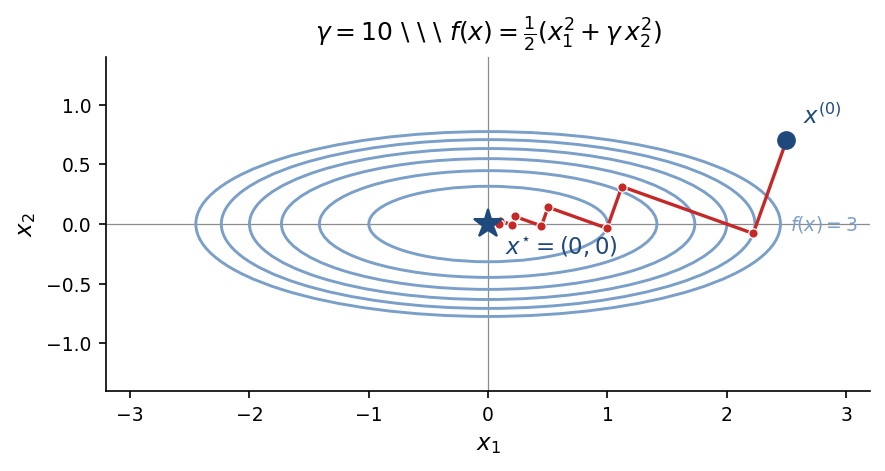
\includegraphics[width=\linewidth]{cap9_images/gradient_zigzag_quadratic.png}
      \end{center}
      \begin{center}\scriptsize \textbf{Zig-zag}: búsqueda exacta sobre $f$ mal condicionada.\end{center}
    \end{column}
  \end{columns}
  \begin{center}
    \scriptsize Cuadrática $f(x)=\tfrac{1}{2}(x_1^2+\gamma x_2^2)$ con búsqueda exacta.
    Pasos siempre ortogonales a los anteriores (gradiente conjugado\newline{} en
    2D, pero la convergencia es \emph{sublineal} en general).
  \end{center}
\end{frame}

\begin{frame}{9.3 Convergencia del descenso por gradiente}
  \begin{theorem}[Velocidad lineal]
    Si $f$ es \textbf{convexa} y de \textbf{Lipschitz con constante $L$} en su gradiente
    ($\nabla f$ es $L$-Lipschitz), entonces con paso $t \le 1/L$ se cumple
    \[
      f(x^{(k)}) - p^{\star} \;\le\; \frac{\|x^{(0)} - x^{\star}\|_{2}^{2}}{2\, t\, k}.
    \]
    Si además $f$ es $m$-\emph{fuertemente convexa}, la convergencia es \textbf{lineal}:
    \[
      f(x^{(k)}) - p^{\star} \;\le\; c^{k}\bigl(f(x^{(0)}) - p^{\star}\bigr),
      \qquad c < 1.
    \]
  \end{theorem}
  \begin{itemize}
    \item El factor $c$ depende de la \emph{razón de condición} $\kappa = L/m$.
    \item Mal condicionamiento ($\kappa$ grande) $\Rightarrow$ zig-zag y convergencia muy lenta.
  \end{itemize}
\end{frame}

% ============================================================
\section{Máximo descenso (steepest descent)}
% ============================================================
\begin{frame}{9.4 Método del máximo descenso}
  \begin{block}{Dirección normalizada}
    Dada una norma $\|\cdot\|$, la dirección de máximo descenso en $x$ es
    \[
      \Delta x_{\mathrm{nsd}} \;=\; \argmin_{\|v\|=1}\; \nabla f(x)^{\top} v.
    \]
    Con $\|\cdot\|_{2}$, $\Delta x_{\mathrm{nsd}} = -\nabla f(x)$ y se recupera el descenso
    por gradiente.
  \end{block}
  \begin{itemize}
    \item \textbf{Con $\|\cdot\|_{1}$:} el método elige un \emph{coordenada} $i$ con
          $|\partial f/\partial x_{i}| = \|\nabla f(x)\|_{\infty}$ y se mueve en $-e_{i}$
          (o $+e_{i}$ según el signo).
    \item \textbf{Con $\|\cdot\|_{\infty}$:} $\Delta x_{\mathrm{nsd}}$ es un vector con
          componentes $-\operatorname{sgn}(\partial f/\partial x_{i})$.
    \item Todas estas normas son \textbf{invariantes bajo escalado}: reescalar las
          coordenadas no cambia la dirección.
  \end{itemize}
  \begin{center}
    \begin{tikzpicture}[scale=0.6, every node/.style={font=\scriptsize}]
      \draw[thick, accentblue!50] (0,0) ellipse (2.5 and 0.9);
      \fill[accentblue!15, opacity=0.6] (0,0) ellipse (2.5 and 0.9);
      \draw[->,thick] (0,0)--(2.7,0) node[above right]{$v$};
      \draw[->,thick,accentred] (0,0)--(1.7,0.6) node[above]{$-\nabla f(x)$};
      \node[accentblue] at (0,1.4) {elipse $\|\cdot\|=1$};
    \end{tikzpicture}
  \end{center}
\end{frame}

% ============================================================
\section{Método de Newton}
% ============================================================
\begin{frame}{9.4 Ejemplo: máximo descenso con $\|\cdot\|_\infty$}
  \begin{example}
    $f(x_1,x_2) = \tfrac{1}{2}(x_1^2 + 2x_2^2)$, $x=(2,1)$, $\nabla f(x) = (2,2)$.
    \[
      \Delta x_{\mathrm{nsd}} = -\operatorname{sgn}(\nabla f(x)) = (-1,-1).
    \]
    \emph{Interpretación:} en cada paso se mueve una unidad a lo largo de
    un eje de coordenadas --- en 2D esto da 4 pasos en zig-zag desde $(2,1)$
    hasta $(0,0)$.
  \end{example}
  \begin{flushright}
    \begin{tikzpicture}[scale=0.5, every node/.style={font=\scriptsize}]
      \draw[->] (-0.4,0)--(3.2,0) node[right]{$x_1$};
      \draw[->] (0,-0.4)--(0,2.4) node[above]{$x_2$};
      \foreach \r in {0.5,1.0,1.5,2.0,2.5} {
        \draw[accentblue!50] (0,0) circle (\r);
      }
      \draw[accentred,->,thick] (2,1) -- (1,1);
      \draw[accentred,->,thick] (1,1) -- (1,0);
      \draw[accentred,->,thick] (1,0) -- (0,0);
      \fill[accentred] (2,1) circle (3pt);
      \fill[accentred] (0,0) circle (3pt);
      \node[accentblue] at (0,2.15) {contornos};
    \end{tikzpicture}
  \end{flushright}
\end{frame}

\begin{frame}{9.5 Método de Newton}
  \begin{block}{Construcción}
    En $x$, aproximar $f$ por su desarrollo de Taylor de 2.\textsuperscript{o} orden:
    \[
      \hat f(x+v) \;=\; f(x) + \nabla f(x)^{\top} v + \tfrac{1}{2}\, v^{\top} \Hess(x)\, v.
    \]
    Minimizando $\hat f$ (asumiendo $\Hess(x) \succ 0$) se obtiene la
    \textbf{dirección de Newton}:
    \[
      \Delta x_{\mathrm{nt}} \;=\; -\Hess(x)^{-1}\, \nabla f(x).
    \]
    El paso es $x^{+} = x + t\, \Delta x_{\mathrm{nt}}$, con $t$ elegido por búsqueda de línea.
  \end{block}
  \begin{itemize}
    \item \textbf{Paso puro} de Newton ($t=1$) es óptimo cerca del óptimo.
    \item \textbf{Decremento de Newton:}
          $\lambda(x) = \bigl(\nabla f(x)^{\top} \Hess(x)^{-1} \nabla f(x)\bigr)^{1/2}$.
          Sirve como criterio de paro ($\lambda^{2}/2 \le \epsilon$).
  \end{itemize}
\end{frame}

\begin{frame}{9.5 Dirección de Newton: geometría}
  \begin{columns}[T]
    \begin{column}{0.5\textwidth}
      \begin{itemize}
        \item La dirección de Newton en $x$ apunta al \emph{mínimo de la
              aproximación cuadrática} de $f$ alrededor de $x$.
        \item Para una cuadrática exacta, ese mínimo es $x^\star$: un solo
              paso de Newton ($t=1$) resuelve el problema.
        \item En general, $\Delta x_{\mathrm{nt}}$ apunta al
              \textbf{centro del elipsoide} de nivel
              $\{v : \nabla f^\top v + \tfrac{1}{2}v^\top\Hess\, v = 0\}$,
              no necesariamente al óptimo.
      \end{itemize}
    \end{column}
    \begin{column}{0.5\textwidth}
      \begin{center}
        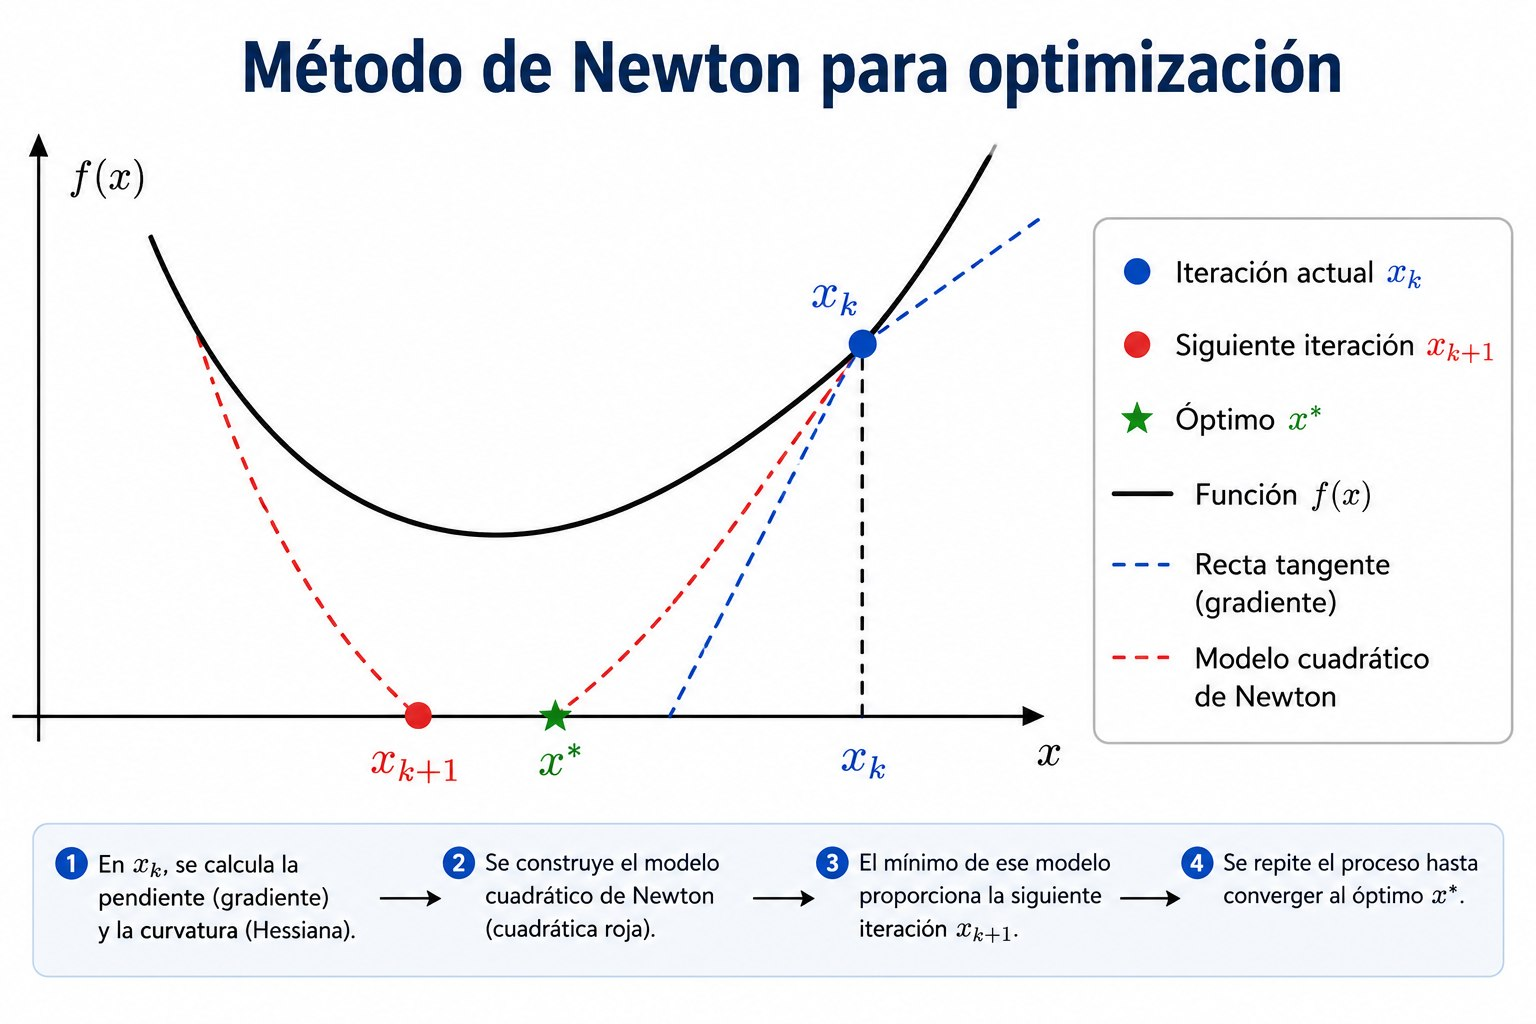
\includegraphics[width=\linewidth]{cap9_images/newton_4_steps.jpg}
      \end{center}
    \end{column}
  \end{columns}
  \begin{center}\scriptsize
    En cada iteración, Newton minimiza el modelo cuadrático local de $f$
    para obtener el siguiente punto.
  \end{center}
\end{frame}

\begin{frame}{9.5 Gradiente vs.\ Newton en un valle estrecho}
  \begin{columns}[T]
    \begin{column}{0.5\textwidth}
      \begin{center}\textbf{Descenso por gradiente}\end{center}
      \begin{tikzpicture}[scale=0.5, every node/.style={font=\scriptsize}]
        \draw[->] (-4.5,0)--(4.8,0) node[right]{$x_1$};
        \draw[->] (0,-2.2)--(0,2.5) node[above]{$x_2$};
        \foreach \r in {0.6,1.2,1.8,2.4,3.0,3.6} {
          \draw[accentblue!50] ({\r*0.97},0) ellipse ({\r*0.97} and {\r*0.20});
        }
        \draw[accentred,->,thick] (3.5,0) -- (0,0.6);
        \draw[accentred,->,thick] (0,0.6) -- (3.0,0);
        \draw[accentred,->,thick] (3.0,0) -- (0,0.3);
        \draw[accentred,->,thick] (0,0.3) -- (1.8,0);
        \draw[accentred,->,thick] (1.8,0) -- (0,0.15);
        \draw[accentred,->,thick] (0,0.15) -- (1.0,0);
        \fill[accentred] (3.5,0) circle (2.5pt);
        \fill[accentred] (0,0) circle (2.5pt);
      \end{tikzpicture}
      \begin{center}\scriptsize \textbf{Muchos pasos}: zig-zag, tasa lineal.\end{center}
    \end{column}
    \begin{column}{0.5\textwidth}
      \begin{center}\textbf{Método de Newton}\end{center}
      \begin{tikzpicture}[scale=0.5, every node/.style={font=\scriptsize}]
        \draw[->] (-4.5,0)--(4.8,0) node[right]{$x_1$};
        \draw[->] (0,-2.2)--(0,2.5) node[above]{$x_2$};
        \foreach \r in {0.6,1.2,1.8,2.4,3.0,3.6} {
          \draw[accentblue!50] ({\r*0.97},0) ellipse ({\r*0.97} and {\r*0.20});
        }
        \draw[accentred,->,very thick] (3.5,0) -- (0,0);
        \fill[accentred] (3.5,0) circle (2.5pt);
        \fill[accentred] (0,0) circle (2.5pt);
        \node[accentred] at (2.0,0.5) {$\Delta x_{\mathrm{nt}}$};
      \end{tikzpicture}
      \begin{center}\scriptsize \textbf{Un solo paso} resuelve la cuadrática.\end{center}
    \end{column}
  \end{columns}
  \begin{center}\scriptsize
    Cuadrática mal condicionada: Newton es \emph{invariante afín},
    gradiente no.
  \end{center}
\end{frame}

\begin{frame}{9.5 Convergencia del método de Newton}
  \begin{theorem}[Convergencia local cuadrática]
    Sea $f \in \mathcal{C}^{3}$ y $x^{\star}$ con $\Hess(x^{\star}) \succ 0$.
    Entonces $x^{(k)}$ generado por Newton ($t = 1$) converge a $x^{\star}$ si
    $x^{(0)}$ está \emph{suficientemente cerca}, y
    \[
      \|x^{(k+1)} - x^{\star}\|_{2} \;\le\; c\,\|x^{(k)} - x^{\star}\|_{2}^{2}.
    \]
  \end{theorem}
  \begin{itemize}
    \item \textbf{Ventaja:} convergencia muy rápida (cuadrática) cerca del óptimo.
    \item \textbf{Desventaja:} cada paso cuesta $\mathcal{O}(n^{3})$ (resolver sistema
          lineal) y construye la Hessiana.
    \item \emph{Sin Hessiana exacta}: Newton-CG, L-BFGS, etc. resuelven
          $\Hess(x)\, \Delta x = -\nabla f(x)$ aproximadamente.
  \end{itemize}
\end{frame}

% ============================================================
\section{Autoconcordancia}
% ============================================================
\begin{frame}{9.6 Funciones auto-concordantes --- motivación}
  \begin{block}{Problema}
    La convergencia cuadrática de Newton requiere estar "cerca" del óptimo, pero
    ¿\emph{qué tan cerca}? y ¿\emph{cómo afecta} el escalamiento de $f$?
  \end{block}
  \begin{itemize}
    \item El análisis clásico usa $m$ y $L$ de la Hessiana, que \emph{no son invariantes}
          bajo transformaciones afines de $x$.
    \item La \textbf{auto-concordancia} (Nesterov--Nemirovski) es una propiedad que
          \textbf{sí} es invariante bajo cambio afín de variable.
    \item Permite cuantificar el número de iteraciones de Newton de forma
          independiente del escalamiento del problema.
  \end{itemize}
\end{frame}

\begin{frame}{9.6 Ejemplo: $f(x) = -\log x$ es auto-concordante}
  \begin{columns}[T]
    \begin{column}{0.5\textwidth}
      Para $f(x) = -\log x$ en $(0,\infty)$:
      \begin{align*}
        f'(x) &= -1/x, \\
        f''(x) &= 1/x^{2}, \\
        f'''(x) &= -2/x^{3}.
      \end{align*}
      Verificamos la desigualdad:
      \[
        |f'''(x)| = \frac{2}{x^{3}} \le 2\left(\frac{1}{x^{2}}\right)^{3/2}
        = 2\, f''(x)^{3/2}.
      \]
      \emph{Igualmente}, $f(x) = -\log(-x)$ en $(-\infty,0)$.
    \end{column}
    \begin{column}{0.5\textwidth}
      \begin{center}
        \begin{tikzpicture}[scale=0.55, every node/.style={font=\scriptsize}]
          \draw[->] (-0.4,0)--(4.5,0) node[right]{$x$};
          \draw[->] (0,-2.5)--(0,3.0) node[above]{$f(x)$};
          % function: -log(x) + small offset
          \draw[thick, accentblue, domain=0.4:4.2, samples=60, smooth]
            plot (\x, {-ln(\x)+0.4}) node[right, black]{$-\log x$};
          % Vertical asymptote
          \draw[dashed, accentred] (0,-2.5) -- (0,3.0) node[above, accentred]{$\dom=(0,\infty)$};
          % Second derivative sample
          \draw[thick, accentgreen!60!black, domain=0.5:3.5, samples=40, smooth]
            plot (\x, {1.2/\x/\x}) node[right, black]{$f''(x)=1/x^{2}$};
        \end{tikzpicture}
      \end{center}
    \end{column}
  \end{columns}
  \begin{center}\scriptsize
    $f''$ cambia rápidamente cerca de la frontera del dominio: por eso
    el método de Newton debe \emph{dar pasos amortiguados} cerca de la frontera.
  \end{center}
\end{frame}

\begin{frame}{9.6 Definición (funciones $\R \to \R$)}
  \begin{definition}[Auto-concordante]
    Sea $f:\R \to \R$ tres veces diferenciable. Decimos que $f$ es \emph{auto-concordante}
    en un intervalo $C \subseteq \dom f$ si
    \[
      |f'''(x)| \;\le\; 2\, f''(x)^{3/2}
      \qquad \text{para todo } x \in C.
    \]
  \end{definition}
  \begin{itemize}
    \item Si la desigualdad vale en $C$ y $f$ es convexa, $f$ se extiende a
          una función auto-concordante en todo su dominio.
    \item \textbf{Ejemplos:} $f(x) = -\log x$ en $(0,\infty)$ y $f(x) = -\log(-x)$
          en $(-\infty,0)$.
  \end{itemize}
\end{frame}

\begin{frame}{9.6 Definición general ($f:\R^{n}\to\R$)}
  \begin{definition}[Auto-concordante en $\R^{n}$]
    $f$ es \emph{auto-concordante} en un conjunto convexo abierto $C$ si para todo
    $x \in C$ y toda dirección $h$, la restricción
    $\varphi(t) = f(x + t h)$ satisface
    \[
      |\varphi'''(0)| \;\le\; 2\, \varphi''(0)^{3/2}.
    \]
  \end{definition}
  \begin{theorem}[Acotaciones de la Hessiana]
    Si $f$ es auto-concordante y $\delta = \bigl(h^{\top} \Hess(x)\, h\bigr)^{1/2} < 1$,
    entonces
    \[
      (1-\delta)^{2}\, \Hess(x) \;\preceq\; \Hess(x+h) \;\preceq\;
      \frac{1}{(1-\delta)^{2}}\, \Hess(x).
    \]
  \end{theorem}
  \begin{itemize}
    \item La cantidad $\delta = \|h\|_{x}$ es la \textbf{norma local} inducida por $\Hess(x)$.
  \end{itemize}
\end{frame}

\begin{frame}{9.6 Complejidad de Newton}
  \begin{theorem}[Conteo de iteraciones]
    Sea $f$ auto-concordante con $\Hess \succ 0$ y sea $x^{(0)}$ con
    $\|x^{(0)} - x^{\star}\|_{x^{(0)}} \le 1$. Entonces Newton con paso
    amortiguado $t = 1$ converge a $x^{\star}$ y el número de iteraciones
    para alcanzar $\lambda(x) \le \epsilon$ es
    \[
      \mathcal{O}\!\bigl(\log\log(1/\epsilon)\bigr).
    \]
  \end{theorem}
  \begin{itemize}
    \item Esta cota es \emph{invariante} bajo reescalamientos afines: depende sólo de
          $\epsilon$, no de constantes de la Hessiana.
    \item A diferencia del teorema clásico de Newton (cuadrática, \emph{local}), aquí
          se obtiene un conteo global gracias a la auto-concordancia.
  \end{itemize}
\end{frame}

% ============================================================
\section{Implementación}
% ============================================================
\begin{frame}{9.7 Implementación de los métodos de descenso}
  \begin{block}{Esquema general}
    \begin{enumerate}
      \item Dado $x$, calcular $f$, $\nabla f$ y (si es Newton) $\Hess$.
      \item Determinar una dirección de descenso $\Delta x$.
      \item Elegir $t$ por búsqueda de línea (exacta o por retroceso).
      \item Actualizar $x \leftarrow x + t \Delta x$.
      \item Repetir hasta $\|\nabla f(x)\| \le \epsilon$ o $\lambda(x) \le \epsilon$.
    \end{enumerate}
  \end{block}
\end{frame}

\begin{frame}{9.7 Detalles prácticos}
  \begin{itemize}
    \item \textbf{Gradiente vs.\ Newton:} gradiente es $\mathcal{O}(n)$ por iteración pero
          converge lineal; Newton es $\mathcal{O}(n^{3})$ pero converge cuadráticamente.
    \item \textbf{Newton sin Hessiana exacta:} métodos cuasi-Newton (BFGS, L-BFGS)
          aproximan $\Hess$ usando diferencias de gradientes --- prácticos
          en dimensiones altas.
    \item \textbf{Búsqueda de línea:} usar \emph{retroceso} (Armijo) salvo que se tenga
          una razón clara para búsqueda exacta (e.g.\ cuadráticas).
    \item \textbf{Criterio de paro:} $\|\nabla f(x)\|_{2} \le \epsilon$ es
          invariante bajo escalado; $f(x^{(k)}) - f(x^{(k-1)}) \le \epsilon$ no lo es.
    \item \textbf{Condicionamiento:} mal condicionado $\kappa = L/m$ grande
          ralentiza el descenso por gradiente --- precondicionar o usar Newton.
  \end{itemize}
\end{frame}

% ============================================================
\section{Resumen}
% ============================================================
\begin{frame}{9.7 Tabla comparativa}
  \begin{center}
    \renewcommand{\arraystretch}{1.3}
    \begin{tabular}{@{}lcccc@{}}
      \toprule
      \textbf{Método} & \textbf{Costo / iter.} & \textbf{Convergencia} & \textbf{Global} & \textbf{Inv. afín} \\
      \midrule
      Gradiente
        & $\mathcal{O}(n)$
        & lineal $c^{k}$ con $c\!\approx\!({\kappa-1})/({\kappa+1})$
        & sí
        & no \\
      Newton
        & $\mathcal{O}(n^{3})$
        & cuadrática local
        & no (sin amortiguam.)
        & sí \\
      Newton amortiguado
        & $\mathcal{O}(n^{3})$
        & cuadrática local
        & sí (búsqueda de línea)
        & sí \\
      Cuasi-Newton (BFGS)
        & $\mathcal{O}(n^{2})$
        & superlineal
        & sí
        & no \\
      Newton + auto-concord.
        & $\mathcal{O}(n^{3})$
        & $\mathcal{O}(\log\log(1/\epsilon))$
        & sí
        & sí \\
      \bottomrule
    \end{tabular}
  \end{center}
  \begin{center}\scriptsize
    $\kappa = L/m$ es la razón de condición de $\nabla^{2} f$ en el óptimo.
  \end{center}
\end{frame}

\begin{frame}{Resumen del capítulo}
  \begin{center}
    \begin{tabular}{@{}lp{6.5cm}@{}}
      \toprule
      \textbf{Método} & \textbf{Características} \\
      \midrule
      Descenso por gradiente
        & $t \le 1/L$; simple; convergencia lineal; zig-zag si mal condicionado. \\
      Máximo descenso
        & Usa $\|\cdot\|$ distinta de $\ell_{2}$; invariante al escalado. \\
      Newton
        & Usa Hessiana; convergencia \emph{cuadrática local}; caro $\mathcal{O}(n^{3})$. \\
      Auto-concordancia
        & Propiedad invariante; garantiza convergencia global de Newton
          en $\mathcal{O}(\log\log(1/\epsilon))$ iteraciones. \\
      \bottomrule
    \end{tabular}
  \end{center}
\end{frame}

\begin{frame}{Referencias}
  \begin{itemize}
    \item S. Boyd and L. Vandenberghe, \emph{Convex Optimization}, Cambridge University Press, 2004.
          \textbf{Capítulo 9: Unconstrained minimization}.
    \item Apuntes de clase y \emph{slides} del curso EE364a, Stanford University.
    \item Y. Nesterov and A. Nemirovskii, \emph{Interior-Point Polynomial Algorithms in Convex Programming},
          SIAM, 1994 (auto-concordancia).
  \end{itemize}
  \vspace{1em}
  \begin{center}
    \emph{Fin de la presentación.}
  \end{center}
\end{frame}

\end{document}
